\begin{frame}{Merge Sort: 먼저 반으로 나눈다}
\mission{각 절반을 정렬한 뒤, 두 정렬된 sequence를 선형 시간에 합친다.}
\centering\begin{tikzpicture}[node distance=5mm]
\node[tree node,minimum width=55mm](a){29 10 14 37 13 5 21 8};
\node[tree node,below left=of a](l){29 10 14 37};\node[tree node,below right=of a](r){13 5 21 8};
\node[sort active,below=of l,minimum width=36mm](sl){10 14 29 37};
\node[sort active,below=of r,minimum width=36mm](sr){5 8 13 21};
\node[chosen,below=8mm of $(sl)!0.5!(sr)$](out){5 8 10 13 14 21 29 37};
\draw[-Latex](a)--(l);\draw[-Latex](a)--(r);
\draw[-Latex](l)--node[left,font=\small]{recursive sort}(sl);
\draw[-Latex](r)--node[right,font=\small]{recursive sort}(sr);
\draw[-Latex,AlgoOrange,very thick](sl)--(out);\draw[-Latex,AlgoOrange,very thick](sr)--(out);
\end{tikzpicture}
\end{frame}
\begin{frame}{MERGE-SORT 의사코드}
\begin{algorithmic}[1]\Procedure{MergeSort}{$A,low,high$}\If{$low\ge high$}\State \Return\EndIf\State $mid\gets low+\left\lfloor\dfrac{high-low}{2}\right\rfloor$\State \Call{MergeSort}{$A,low,mid$}\State \Call{MergeSort}{$A,mid+1,high$}\State \Call{Merge}{$A,low,mid,high$}\EndProcedure\end{algorithmic}
\begin{block}{안전한 midpoint}$low+\lfloor(high-low)/2\rfloor$는 $low+high$의 정수 overflow를 피한다.\end{block}
\end{frame}
\begin{frame}{MERGE의 Mission}
\mission{\texttt{Merge(A,low,mid,high)}는 정렬된 두 구간 $A[low..mid]$, $A[mid+1..high]$를 $A[low..high]$에 안정적으로 합친다.}
\[L=[10,14,29,37],\quad R=[5,8,13,21]\]
각 원소는 정확히 한 번 output으로 이동하므로 $\Theta(|L|+|R|)$이다.
\end{frame}
\begin{frame}{MERGE 의사코드}
\small\begin{algorithmic}[1]
\Procedure{Merge}{$A,low,mid,high$}
\State $L\gets A[low..mid]$; $R\gets A[mid+1..high]$
\State $i,j\gets1,1$; $k\gets low$
\While{$i\le |L|$ and $j\le |R|$}
\If{$L[i]\le R[j]$}\State $A[k]\gets L[i]$; $i\gets i+1$
\Else\State $A[k]\gets R[j]$; $j\gets j+1$\EndIf
\State $k\gets k+1$
\EndWhile
\State copy the remaining suffix of $L$ or $R$ into $A[k..high]$
\EndProcedure
\end{algorithmic}
\vfill\muted{$L[i]=R[j]$이면 왼쪽 record를 먼저 선택하므로 relative order가 보존된다.}
\end{frame}
\begin{frame}{MERGE: 두 Pointer만 전진한다}
\centering\begin{tikzpicture}[x=.95cm,y=1cm]
\node[font=\bfseries,anchor=east]at(-.6,1){L};\node[font=\bfseries,anchor=east]at(-.6,0){R};\node[font=\bfseries,anchor=east]at(-.6,-1.2){out};
\foreach \x/\v in {0/10,1/14,2/29,3/37}\node[sort cell]at(\x,1){\v};
\foreach \x/\v in {0/5,1/8,2/13,3/21}\node[sort cell]at(\x,0){\v};
\only<1>{\def\out{{{},{},{},{},{},{},{},{}}}\node[sort current]at(0,0){5};}
\only<2>{\def\out{{5,8,{},{},{},{},{},{}}}\node[sort current]at(0,1){10};}
\only<3>{\def\out{{5,8,10,13,{},{},{},{}}}\node[sort current]at(1,1){14};}
\only<4>{\def\out{{5,8,10,13,14,21,29,37}}}
\foreach \i in {0,...,7}{\pgfmathparse{\out[\i]}\edef\v{\pgfmathresult}\node[sort done]at(\i,-1.2){\v};}
\end{tikzpicture}
\vspace{2mm}\only<1|handout:0>{5부터 선택}\only<2|handout:0>{5, 8 뒤에는 10}\only<3|handout:0>{13 다음 14}\only<4|handout:1>{한쪽이 비면 나머지 suffix를 붙인다.}
\end{frame}
\begin{frame}{Merge Sort의 시간}
\begin{columns}\column{.5\textwidth}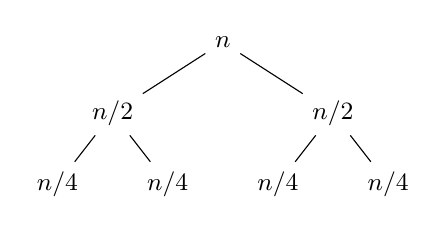
\begin{tikzpicture}[level distance=9mm,level 1/.style={sibling distance=28mm},level 2/.style={sibling distance=14mm},every node/.style={font=\small}]
\node{$n$}child{node{$n/2$}child{node{$n/4$}}child{node{$n/4$}}}child{node{$n/2$}child{node{$n/4$}}child{node{$n/4$}}};\end{tikzpicture}\column{.47\textwidth}각 level의 merge 비용은 $\Theta(n)$, level 수는 $\Theta(\log n)$.\[T(n)=\Theta(n\log n)\]\end{columns}
\end{frame}
\begin{frame}{Merge Sort Takeaway}
\begin{itemize}\item 길이 $n$ segment의 merge는 $\Theta(n)$\item best = average = worst: $\Theta(n\log n)$\item stable; 배열 구현은 보통 $\Theta(n)$ buffer와 $\Theta(\log n)$ recursion stack을 사용하며 buffer가 지배한다.\item linked list와 external sorting에 특히 자연스럽다.\end{itemize}
\sortingtakeaway{예측 가능한 시간과 stability를 얻는 대신 추가 공간을 사용한다.}
\muted{Merge Sort는 균형 있게 먼저 나누고 나중에 합친다. Quick Sort는 partition 결과에 따라 분할 크기가 결정된다.}
\end{frame}
